\documentclass{beamer}[10]


%
% macro
%


% Set par-tec and event logo
\newcommand{\mainlogo}{
    \hspace{5pt}
\includegraphics[height=1cm]{par-tec-logo.png}
}
\newcommand{\eventlogo}{
    \hspace{210pt}\includegraphics[height=1.2cm]{}
}

\usepackage{pgf}
\usepackage[english]{babel}
\usepackage[utf8]{inputenc} % use unicode chars
\usepackage{lmodern}% http://ctan.org/pkg/lm
\usepackage{bashful} % execute scripts inside latex and create dynamic .tex files
\usepackage{beamerthemesplit}
\usepackage{color}
\usepackage{graphics,epsfig,subfigure}
\usepackage{hyperref}
\usepackage{import}
\usepackage[mathescape,escapeinside=||]{minted}
\usepackage{mathtools}
\usepackage{makeidx}
\usepackage{multicol}
\usepackage{mdframed}
\usepackage{url}
\usepackage{srcltx}
\usepackage{amsmath}
%\usepackage[beamer]{hf-tikz}
\usepackage{xfrac}
\usepackage{ragged2e} % text alignment

%
% Packages for markdown conversion
%
\usepackage{amssymb}
%\usepackage{ifxetex}
%\usepackage{ifluatex}
\usepackage{listings}
\usepackage{fancyvrb}
\usepackage{longtable}
\usepackage{booktabs}
\usepackage{graphicx}
\usepackage{ulem}
%\usepackage{fontspec}
%\usepackage{xltxtra}
\usepackage{xunicode}


%\showboxdepth=5
%\showboxbreadth=5

% Slides in 16:9
\usepackage[orientation=landscape,size=custom,width=16,height=9,scale=0.5,debug]{beamerposter}

%
% Macros
%
\definecolor{darkred}{rgb}{0.55, 0.0, 0.0}
\definecolor{light-gray}{gray}{.80}
\definecolor{light-yellow}{rgb}{255,255,153}
\definecolor{alizarin}{rgb}{0.82, 0.1, 0.26}
% colorized font
\newcommand{\red}[1] {{\color{red} #1}}
\newcommand{\darkred}[1] {{\color{darkred} #1}}
\newcommand{\blue}[1] {{\color{blue} #1}}
\newcommand{\green}[1] {{\color{green} #1}}
\newcommand{\gray}[1] {{\color{gray} #1}}
\newcommand{\grey}[1] {{\color{gray} #1}}

\newcommand{\hearts} {\red{$\heartsuit$}}
\newcommand{\diamonds} {\red{$\diamondsuit$}}
\newcommand{\spades} {$\spadesuit$}
\newcommand{\clubs} {$\clubsuit$}
\newcommand{\pyoptional}[1]{\diamonds #1 \diamonds}

\newcommand{\deltasum}[1]{\sum (#1 - \bar{#1})}
\newcommand{\deltasumsq}[1]{\sum (#1 - \bar{#1})^{2}}

%
% Take care of the newline after \frametitle
%
\newenvironment{pyframe}[1]
{\begin{frame}[fragile,environment=pyframe]\frametitle{#1}

}
{\end{frame}}


% environments
\newminted{py}{mathescape,escapeinside=||}%
\newminted{bash}{mathescape,fontsize=\small}%

% python highlights: module, method
\newcommand{\pymodule}[1]{\darkred{\textbf{#1}}}
\newcommand{\pyfunction}[1]{\textit{#1}}
\newcommand{\keyword}[1]{\texttt{#1}}
\newcommand{\pyver}[1]{\colorbox{yellow}{#1}}
\newcommand{\typeonly}[1]{\colorbox{green}{#1}}
\newcommand{\pyvers}[1]{\raisebox{0em}{\colorbox{yellow}{#1}}}
\newcommand{\code}[1] { \texttt{#1} }
% support for columns in markdown
\newcommand{\columnsbegin}{\begin{columns}}
\newcommand{\columnsend}{\end{columns}}
%support for minted in markdown
%\newcommand{\pythonbegin}{\begin{pycode*}}
%\newcommand{\pythonend}{\end{pycode*}}

% special symbils
\newcommand{\mymapsto}{\operatornamewithlimits{\longmapsto}}

\makeatletter
\newcommand{\xMapsto}[2][]{\ext@arrow 0599{\Mapstofill@}{#1}{#2}}
\def\Mapstofill@{\arrowfill@{\Mapstochar\Relbar}\Relbar\Rightarrow}
\makeatother




%
% style
%

\setbeamercovered{transparent}
\mode<presentation>

%\geometry{top=5pt, margin=5pt}
%The outertheme defines the head and the footline of each slide
% \setbeamercolor{block title}{bg=orange}
% \useinnertheme{circles}
% \useoutertheme{split}
%\beamertemplatenavigationsymbolsempty

%\usetheme[numbers,totalnumber,compress,sidebarshades]{Babel}
\setbeamertemplate{headline}{
 \leavevmode%
  \hbox{%
%,bb=0 0 5cm 2cm
    \mainlogo
    \eventlogo
    }
}
\setbeamertemplate{footline}{
\noindent\textbf{\hspace{5pt}\insertsection \insertsubsection\hfill}\textbf{\hfill{\color{gray}\insertshortauthor}\hfill}\textbf{\hfill }
   % \textline[t]{ \insertsection  \insertsubsection}{\gray{\insertshortauthor}}{right}
}
%\useinnertheme[shadow=false]{rounded}
% frametitle
\setbeamertemplate{frametitle}[default][center]
\setbeamercolor*{frametitle}{bg=white,fg=gray,parent=palette primary}
\setbeamerfont{frametitle}{series=\bfseries,size={\fontsize{16}{8}}}
% table of contents
\setbeamercolor{section in toc}{fg=black} % series=\bfseries,size={\fontsize{16}{8}}}
%\setbeamercolor{section/subsection in toc}{fg=black}
%\setbeamercolor{subsection in toc}{fg=black}
%\setbeamerfont{section in toc}{fg=black} % series=\bfseries,size={\fontsize{16}{8}}}
%\setbeamerfont{section/subsection in toc}{fg=black}
%\setbeamerfont{subsection in toc}{fg=black}

%title
\setbeamercolor{title}{fg=black,bg=white}
\setbeamerfont{title}{series=\bfseries,size={\fontsize{24.88}{32}}}
%subtitle
\setbeamercolor{subtitle}{fg=gray}
\setbeamerfont{subtitle}{series=\bfseries,size={\fontsize{14}{}}}
%titlepage
\setbeamertemplate{title page}[default][center]
% bullets
\setbeamercolor{itemize item}{fg=gray}
\setbeamertemplate{itemize items}[circle]
\setbeamercolor{itemize item}{fg=light-gray}
\setbeamercolor{itemize items}{fg=light-gray}
% enumerations
\setbeamercolor{enumerate item}{fg=black}
\setbeamercolor{local structure}{fg=black}

%
% increase itemize spacing
%
%\newlength{\wideitemsep}
%\setlength{\wideitemsep}{\itemsep}
%\addtolength{\wideitemsep}{14pt}
%\let\olditem\item
%\renewcommand{\item}{\setlength{\itemsep}{\wideitemsep}\olditem}

  % \usecolortheme[named=orange]{structure}
  % \useinnertheme{circles}
  % \usefonttheme[onlymath]{serif}
\setbeamercovered{transparent}
  % \setbeamertemplate{blocks}[rounded][shadow=true]

\makeindex



% Apply DRAFT watermark
\usepackage{draftwatermark}
\setbeamercolor{background canvas}{bg=}%transparent canvas


\title{Python for System Administrator}
%\subtitle{EuroPython 2014, $24^{th}$ July - Berlin}
\author{Roberto Polli - \href{mailto:roberto.polli@par-tec.it}{roberto.polli@par-tec.it}}
%\date{24 July 2014}
\institute{Par-Tec Spa  - Rome Operation Unit \\
    P.zza S. Benedetto da Norcia, 33\\ 
    00040, Pomezia (RM) - www.par-tec.it%
    }

%
%
\begin{document}

%% cover
\frame{\frametitle{}\titlepage
%%\vspace{-0.5cm}
}

%% agenda
\frame{\frametitle{Agenda}
\begin{multicols}{2}
\tableofcontents
\end{multicols}

}

% \section{Test}
\usepackage{pdfcomment}

\begin{pyframe}{Title}
Antani
module: \pymodule{subprocess, psutil}
symbols: $\clubsuit \diamondsuit \heartsuit \spadesuit$
\end{pyframe}

\begin{pyframe}{\pyoptional{Test Slide with styles}}
\begin{itemize}
\item Bullet \index{Bullet} item 0 $a_i + b_j = 10 $
\item Bullet \index{Bullet} item 2 with code\footnote{Do you like footnotes?}
\begin{pycode*}{escapeinside=||}
    # footnotesize
    for  a in range(10):
        yield a
    # $\xmapsto[encode]{utf-8}$
    # $a \rightarrow b^{c}$
    |\index{return}return| False
\end{pycode*}
\item Bullet Item 3 
\end{itemize}
\end{pyframe}

\begin{pyframe}{Test Slide with styles}
\begin{enumerate}
\item Enumerate1 \index{enumerate} \pdfcomment{Pdf Comment Test Slide with styles}
    \begin{enumerate}
    \item EnumerateA  \pyver{w\"urstel re}sults
    \item \texttt{Inline minted ipython}
    \item Una linea 
    \item w\"urstelstra\ss e
    \end{enumerate}

\item Enumerate2 \`{e} 
 [\red{196}, \blue{168}] 
\begin{pycode*}{escapeinside=||}
@|\pyver{decorator}|
def foo(tmp):
    def bar(*args):
        |\index{return}return| tmp(|$*args_{i}$|)
    |\index{return}return| bar
\end{pycode*}

\end{enumerate}

\end{pyframe}

\begin{pyframe}{Tabular and image}
A Tabular follows \\
\begin{tabular}{|c|c|}\hline
Cell 1 & Cell 2 \\
\hline 
\end{tabular}
\\
\begin{table}
\begin{tabular}{|c|c|}\hline
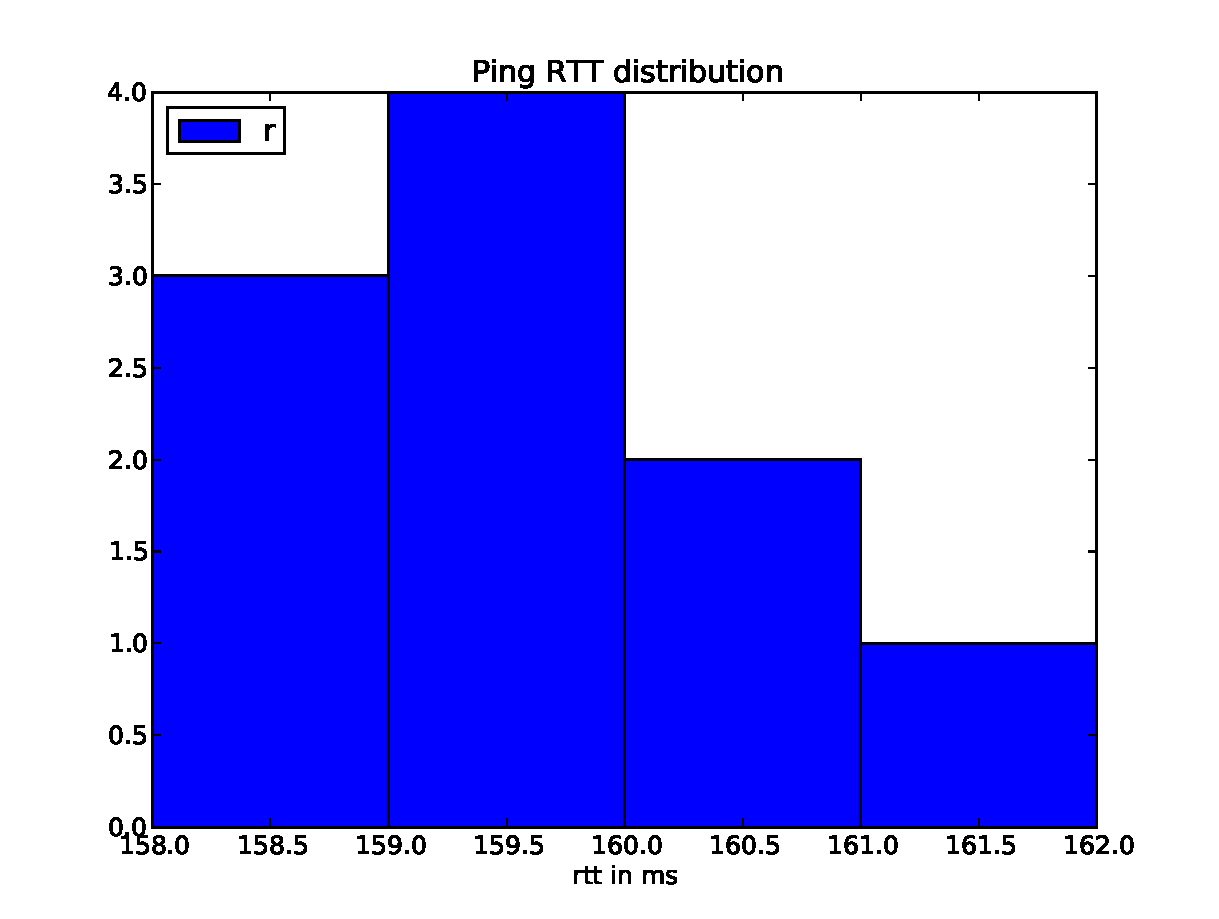
\includegraphics[height=4cm]{ping_distribution.pdf}   & 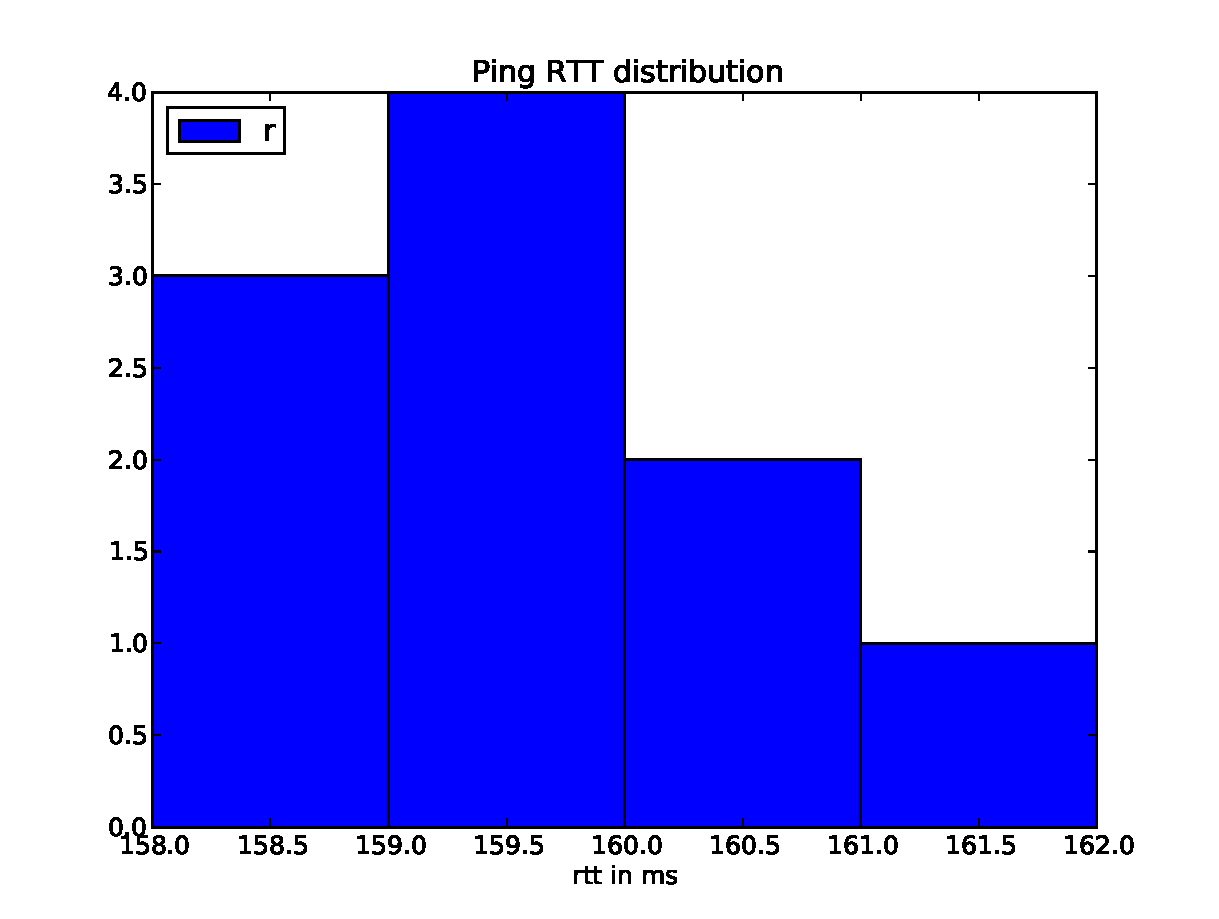
\includegraphics[height=4cm]{ping_distribution.pdf}  \\
\hline 
\end{tabular}
\end{table}
\end{pyframe}

\begin{pyframe}{Simple Column}
\begin{columns}
\column[t]{6cm}
\begin{pycode}
"""using set and dict
"""
distro = {x: rtt.count(x) 
  for x in set(rtt)}
# or using a
from collections import defaultdict
distro = defaultdict(int)
for x in rtt:
    distro[x] += 1
    

\end{pycode}
\column[t]{5cm}
-skip-\\
-skip-\\
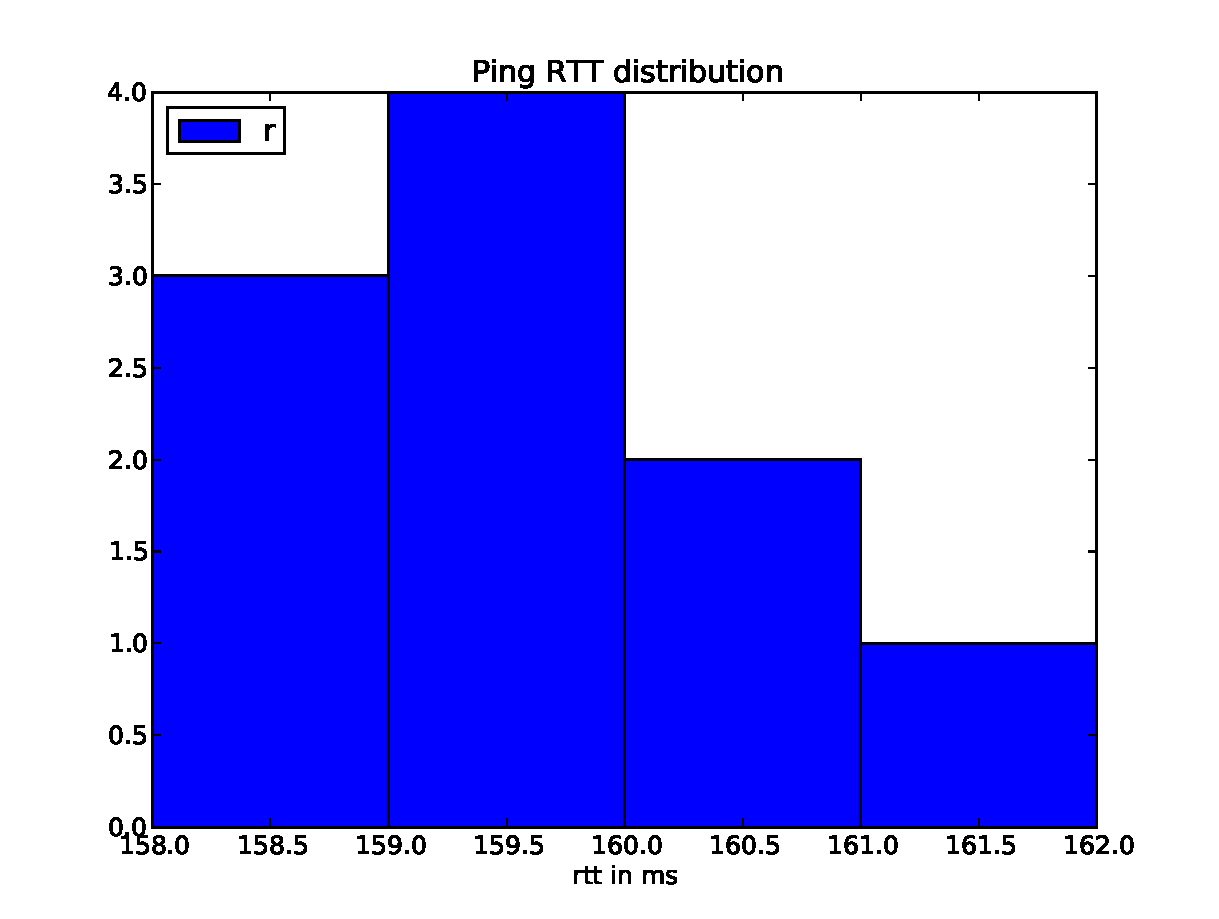
\includegraphics[height=4cm, width=4dm]{ping_distribution.pdf}  
\end{columns}
\end{pyframe}


\begin{pyframe}{2-columns and verbatim}
Two columns
\begin{columns}

\column[t]{5cm}
1
2
3
\begin{verbatim}
4
5
6
\end{verbatim}

\column[t]{5cm}
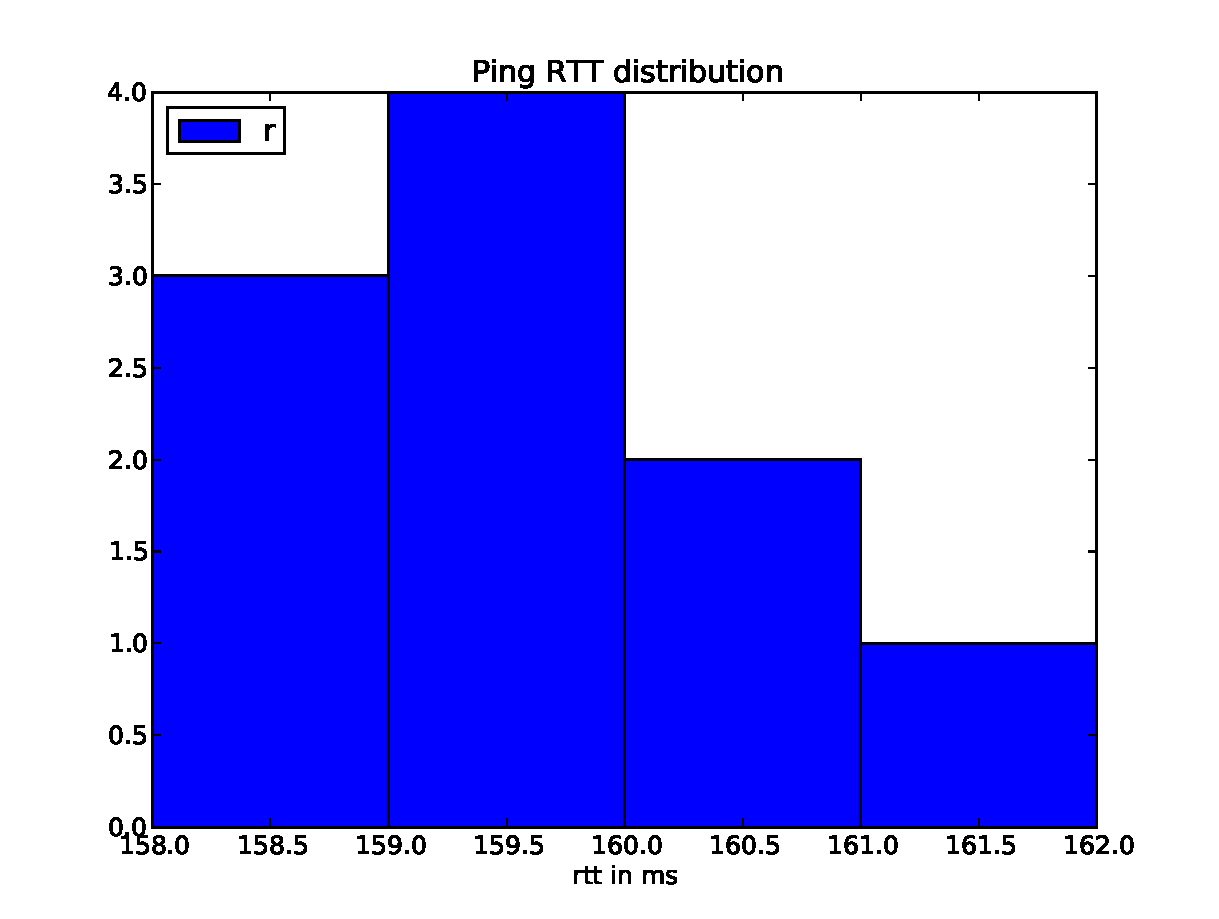
\includegraphics[height=4cm,width=5cm]{ping_distribution.pdf}  
\end{columns}

\end{pyframe}



\begin{pyframe}{Simple processing: distribution}
\begin{columns}
\column[t]{6cm}
\begin{pycode}
"""using set and dict """
distro = {x: rtt.count(x) 
  for x in set(rtt)}
# or using a
from collections import defaultdict
distro = defaultdict(int)
for x in rtt:
    distro[x] += 1
\end{pycode}
\column[t]{4cm}
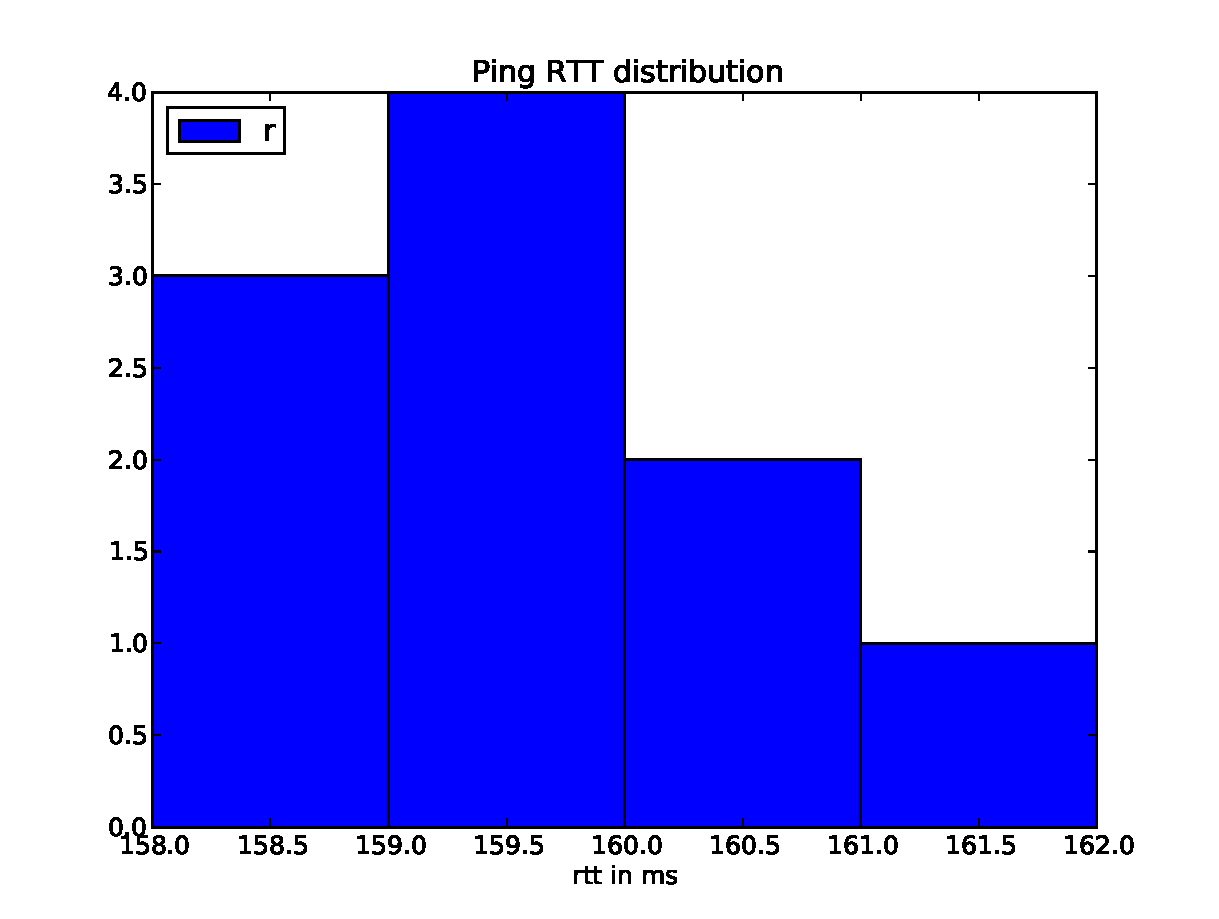
\includegraphics[width=4cm,height=4cm]{ping_distribution.pdf}  
\end{columns}
\end{pyframe}

\begin{pyframe}{Index}

fooo bar

\end{pyframe}



\section{Intro}
\frame{ \frametitle{Who? What? Why?}
\begin{itemize}

\item Use python to replace Grep Awk Sed Perl. Speed up your daily job.
\\

\item Roberto Polli - Solutions Architect @ par-tec.it. Loves writing in C,
Java and Python. Red Hat Certified Engineer and Virtualization
Administrator.
\\

\item Par-Tec – Proud sponsor of this talk ;) Contributes to various FLOSS and
provides expertise in IT Infrastructure \& Services and Business Intelligence
solutions + Vertical Applications for the financial market.

\end{itemize}
}


\begin{pyframe}{Requirements}
\begin{itemize}
\item python 2.7+, ipython

\item course code from github \\\\
\code{ \#git clone https://github.com/ioggstream/python-course}

\item test your environment (eg. psutil, numpy, scipy, matplotlib) \\\\
\code{ \#nosetests -vs test\_prerequisites.py }

\item first part: \pymodule{nose, psutil}
\item second part: \pymodule{scipy, numpy, matplotlib}
\item \pyoptional{optional/advanced content}
\end{itemize}
\end{pyframe}

\frame{ \frametitle{How}
\begin{itemize}
\item Get ready $before$ starting: code is \href{https://github.com/ioggstream/python-course/tree/master/python-for-sysadmin/README}{here on github}!

\item \emph{Type everything} but \code{\#comments} and \code{try/except}

\item \emph{Type fast} with tab-completion and copy-paste
% \emph{Type smart} with \code{\%edit testfile.py}!

\item Be curious: inspect and print returned variables

\item $Never^{*}$ close your iPython session: you'll lose your precious variables

\end{itemize}

* (ok, sometimes you can).
}

\begin{pyframe}{References}
\begin{itemize}
\item irc.freenode.net\# python - The Python Community :D
\item Python Cookbook 3rd ed. O'Reilly - David Beazley and Brian K. Jones
\item Programming Python 4th ed. O'Reilly - Mark Lutz
\item Dive into Python3 2nd ed. Apress - Mark Pilgrim
\item nose.readthedocs.org
\item github.com/ioggstream/python-course
\end{itemize}
\end{pyframe}


\section{ipython}



\begin{frame}{iPython I}
\begin{itemize}
\item an interactive interpreter with tonns of                                                                                                        functionalities, and the main tool of our training.                                                                                                      

\item   It's the funniest way to learn and use python!

\item   Supports tab-completion, inline help and elementary
    benchmarking

\item   Run it: \\
\mintinline{bash}{ipython}
\end{itemize}

\end{frame}


\begin{frame}[fragile]{iPython II}
\begin{minted}[mathescape]{python}
# iPython supports inline-help
#  appending ? to an object
str?

# We can run commands
#  and capture the output in a variable
# don't need to quote using the ! magic
# on unix
ret = !cat /etc/hosts

# windows has etc\hosts too ;)
ret = !type c: windows\system32\drivers\etc\hosts
\end{minted}
\end{frame}


\begin{frame}[fragile]{iPython III}
\begin{minted}[mathescape]{python}
# returned objects can be filtered
#  with its grep and fields methods
ret.grep('localhost')
# return the first space-splitted column of
#  the output
ret.fields(0)
ret.grep('localhost').fields(0)

# And the last returned value is stored in 
localip = _

# An ipython script \empth{must} have the 
#  .ipy extension and begin with
#!/usr/bin/ipython 
\end{minted}
\end{frame}



\section{Path management: 10'}

\begin{frame}[fragile]{Path management: Goal}
\begin{itemize}
\item Normalize paths on different platform
\item Create, copy and remove folders
\item Handle errors
\item modules: \emph{os, os.path, shutil, errno}
\end{itemize}
\end{frame}

\begin{frame}[fragile]{Path management: os.path, sys}
% This slide is the core one. Required for data gathering!
\begin{minted}[mathescape]{python}
hosts, basedir = "etc/hosts", "/"
# Check the hosting platform with the sys module
from sys import platform
if platform.startswith('win'):
    basedir = 'c:/windows/system32/drivers'

# Always use the os.path module!
from os.path import join, normpath 
hosts = join(basedir, hosts)
hosts = normpath(hosts)
print("Normalized path is", hosts)
\end{minted}
\end{frame}

\begin{frame}[fragile]{Path management: os.path, sys}
\Large
\begin{itemize}
\item \emph{os.path} is the best way to manage paths!
\begin{itemize}
 \Large
 \item multiplatform
 \item safe
 \end{itemize}
 
\item os.path.normpath fixes "/" orientation!
\item os.path.join 
 \end{itemize}
And now, let's rapidly see some other tools $\ldots$
\end{frame}

\begin{frame}[fragile]{Move trees: shutil, os, os.path}
\begin{minted}[mathescape]{python}
# os and shutil can perform...
from os import makedirs     # ...tree creation...
from shutil import copytree, rmtree 
makedirs("/tmp/course/foo/bar")

# ...while os.path can test file existence
from os.path import isdir            
assert isdir("/tmp/course/foo/bar")

# copy a whole tree... check it...
copytree("/tmp/course/foo", "/tmp/course/foo2") 
assert isdir("/tmp/course/foo2/bar")            

rmtree("/tmp/course/foo") # ... and delete it
assert not isdir("/tmp/course/foo/bar")
\end{minted}
\end{frame}

\begin{frame}[fragile]{Move trees: errno}
\begin{minted}[mathescape]{python}

# We can use exception handlers to investigate errors
   try:
        # python2 does not allow to ignore
        #  already existing directories
        #  and raises an OSError
        makedirs("/tmp/course/foo/bar")
    except OSError as e:
        # Just use the errno module to
        #  check the error value
        import errno
        assert e.errno == errno.EEXIST
\end{minted}
\end{frame}



\section{Encoding: 10'}

\begin{pyframe}{Encoding: Goal}
\Large
\begin{itemize}
\item A string more than a sequence of bytes
\item \emph{A string is a couple (bytes, encoding)}
\item Use unicode\_literals in python2
\item Manage differently encoded filenames 
\item A string is not a sequence of bytes
\end{itemize}
modules: \pymodule{os, os.path, glob}
\end{pyframe}


\begin{pyframe}{Song of \emph{C}hildhood}
\begin{columns}

\column[c]{.15\textwidth}
\tiny
\textit{Als das Kind Kind war, ging es mit hängenden Armen, 
wollte der Bach sei ein Flu\ss, der Flu\ss sei ein Strom, 
und diese Pf\"utze das Meer.
\newline
Als das Kind Kind war,  wu\sste es nicht, da\ss es Kind war, 
alles war ihm beseelt, und alle Seelen waren eins.
\newline
Als das Kind Kind war, 
hatte es von nichts eine Meinung, 
hatte keine Gewohnheit, 
sa\ss oft im Schneidersitz, 
lief aus dem Stand, 
hatte einen Wirbel im Haar 
und machte kein Gesicht beim fotografieren.
}
\column[c]{.7\textwidth}
\begin{verse}
\begin{center}
\Large
```When the child was a child,\\
\vspace{.5cm}
characters were bytes, and\\
\vspace{.5cm}
strings list of bytes'''
\end{center}
\end{verse}

\column[c]{.15\textwidth}
\tiny \textit{Als das Kind Kind war, 
fielen ihm die Beeren wie nur Beeren in die Hand 
und jetzt immer noch, 
machten ihm die frischen Waln\"usse eine rauhe Zunge 
und jetzt immer noch, 
hatte es auf jedem Berg 
die Sehnsucht nach dem immer h\"oheren Berg, 
und in jeder Stadt 
die Sehnsucht nach der noch gr\"o\sseren Stadt, 
und das ist immer noch so, 
griff im Wipfel eines Baums nach dem Kirschen in einemHochgef\"uhl 
wie auch heute noch, 
eine Scheu vor jedem Fremden 
und hat sie immer noch, 
wartete es auf den ersten Schnee, 
und wartet so immer noch.
}
\end{columns}
\end{pyframe}

\iffalse
\begin{pyframe}{Encoding is a map}
\begin{itemize}
\item The \emph{type()} of a byte-sequence is bytes
\item Encoding is a one-to-one map between a typographical character and a byte-sequence 
\item Decoding is its reverse map
\end{itemize}

\begin{columns}
\column[c]{.6\textwidth}
\begin{pythoncode*}{escapeinside=||}
# heading $\pyver{u}$ only in py2
b1 = |\pyver{u}|"S\u00fcd".encode('utf-8') 
b2 = |\pyver{u}|"S\u00fcd".encode('cp1252')

# it's always true that
type(b1) == type(b2) == bytes
# but only in py2
str == bytes





\end{pythoncode*}

\column[c]{.4\textwidth}
\small
\begin{tabular}{|c||c|c|c|}\hline 
            & \multicolumn{3}{|c|}{bytes}  \\ \hline
char        & ascii     & utf-8         & cp1252     \\ \hline
a           & [97]      & [97]          & [97]      \\ \hline     
$\ddot{u}$  & -         & [195, 188]    & [\pyver{252}]              \\ \hline
\`{e}     &  - & [196, 168] & [232]\\ \hline
\end{tabular}
\end{columns}

\end{pyframe}
\fi
%%
\begin{pyframe}{Encoding is a map}
\begin{columns}
\column[c]{.6\textwidth}


\begin{pythoncode*}{escapeinside=||}
# heading $\pyver{u}$ only in py2
the_string = |\pyver{u}|"S\u00fcd" # $S\"ud$

# can be encoded in different
in_utf8 =  the_string.encode('utf-8')
in_win = the_string.encode('cp1252')

type(in_utf8) == bytes # byte-sequences

# Decoding bytes using the wrong map..
# ...gives weird results
in_utf8.decode('cp1252') # $S\~A\sfrac{1}{4}d$





\end{pythoncode*}

\column[c]{.4\textwidth}
\begin{itemize}
\item Encoding is a one-to-one map between a typographical character and a byte-sequence 
\item Decoding is its reverse map
%\item The \emph{type()} of a byte-sequence is bytes
\end{itemize}

\small
\begin{tabular}{|c||c|c|c|}\hline 
%            & \multicolumn{3}{|c|}{bytes}  \\ \hline
char        & ascii     & utf-8         & cp1252     \\ \hline
a           & [97]      & [97]          & [97]      \\ \hline     
$\ddot{u}$  & -         & [195, 188]    & [252]              \\ \hline
%\`{e}     &  - & [196, 168] & [232]\\ \hline
\end{tabular}
\end{columns}

\end{pyframe}



%%

\iffalse
\begin{pyframe}{De}
\begin{itemize}
\item A string is a couple: (bytes, encoding) 
\item The same string can be encoded using different maps.
\end{itemize}

\begin{table}
\begin{tabular}{|c|l|} \hline 
encoding & the string  S\pyver{\"u}d results in bytes \\ \hline 
utf-8 &([83, \pyver{195, 188}, 100]  \\
cp1252 &([83, \pyver{252}, 100]\\
\hline
\end{tabular}
\end{table}

\begin{verse} \begin{center}
\huge
\"u  {\footnotesize versus}  \~{A}  $\sfrac{1}{4}$
\\
\end{center} \end{verse}

\begin{center}
\Large
\"{u} $\xmapsto[encode]{utf-8}$ 
    [\red{198}, \blue{188}] 
    $\xmapsto[decode]{cp1252}$ 
    \red{\~{A}} \blue{$\sfrac{1}{4}$}
\end{center}

\end{pyframe}
\fi

\begin{pyframe}{Enters Encoding}
\begin{minted}[mathescape]{python}
# Filenames are binary data! $\emph{Be careful}$ when reading from
#  a (eg. vfat) filesystem!
# To make python2 encoding-aware we should
from __future__ import unicode_literals

# Create 3 windows-encoded filenames in 
basedir = "/tmp/course"

# using the provided function
from exercises import create_wuerstelstrasse
create_wuerstelstrasse(basedir)
\end{minted}
\end{pyframe}


\iffalse
\begin{pyframe}{Encoded filenames}
\begin{pythoncode*}{escapeinside=||}
# What happens mangling them with the $\emph{os}$ module?
from os.path import join as pjoin
from os import listdir as ls       # similar to unix ls ;)

list_files_with = ls(basedir)

# ooops! Got an encoding error?
create_full_path = pjoin(basedir, list_files_with[0])

# $\emphred{UnicodeDecodeError:}$ 'ascii' codec can't decode $\pyver{byte 0xFC}$
#    in position 2: ordinal not in range(128)
|\pyver{0xFC}| == 252 # remember the $\"u$ in cp1252 map? 
\end{pythoncode*}
\end{pyframe}

\begin{pyframe}{Encoded filenames II}
\begin{pythoncode*}{escapeinside=||}

# $\emph{os.path}$ on py2 fails mangling those files as encoded strings
#  so we ask it to mangle them as $\emph{bytes}$
bytebasedir = bytes(basedir)

for f in files: # listdir is already safe ;)
    byte_full_path = pjoin(basedir, f)
    # we use $\pyver{"{!r}"}$.format to avoid further encoding
    #     issues when printing or logging
    print("file: {!r}".format(utf_path))
    
\end{pythoncode*}
\end{pyframe}
\fi

\begin{pyframe}{Encoded filenames: glob}
\begin{pythoncode*}{escapeinside=||}
from glob import glob as ls # expands wildcards like a shell. 
files = ls("/tmp/course/*.txt") # To avoid encoding issues ...
# $\red{UnicodeDecodeError:}$ 'ascii' codec can't decode $\pyver{byte 0xFC}$
|\pyver{0xFC}| == 252 # remember the $\"u$ in cp1252 map? 

for f in ls(|\pyver{b}|"/tmp/course/*.txt"):
    try: # ...we explicitly use byte-sequences
        print("file: {!s}".format(f))
    except UnicodeDecodeError as e:
        # and use $\pyver{"{!r}"}$.format to avoid further encoding
        print("Error decoding {!r}".format(f))

\end{pythoncode*}
\end{pyframe}


\begin{pyframe}{Encoded filenames: Complete Example}
\begin{minted}[mathescape]{python}
def list_files(basedir):
    """Works both if isinstance(basedir, unicode)
        or isinstance(basedir, bytes)"""
    for f in ls(basedir):
        try:
            utf_or_byte_path = pjoin(basedir, f)
            print("file: {!s}".format(utf_or_byte_path))
        except UnicodeDecodeError as e:
            print("Error decoding {!r}".format(f))

bytebasedir = bytes(basedir)
list_files(basedir)     # which one ...
list_files(bytebasedir) # ...will work?
    
\end{minted}
\end{pyframe}


\section{Data Gathering: 20'}
%
% NOTE: minted allows mathescape everywhere now;)
%


\begin{pyframe}{Data Gathering: Goal}
    Gathering System Data with multiplatform
     and platform-dependent tools.
\begin{itemize}
\item Get infos from files, /proc and /sys 
\item Run and capture command output
\item Use psutil to get IO, CPU and memory data
\item Parse files with a strategy
\end{itemize}
modules: \pymodule{psutil, subprocess, os}
\end{pyframe}


\begin{pyframe}{Data Gathering: grep}
\begin{pycode}
def grep(needle, fpath):
    """is a minimal grep implementation

       goal: open() is iterable and doesn't
             need splitlines()
       goal: comprehension can filter iterables
    """
    return [x for x in open(fpath) if needle in x]
    
# Do we have "localhost" in our "/etc/hosts"?
grep("localhost", "/etc/hosts")
\end{pycode}
\end{pyframe}

\subsection{module: psutil}
\begin{pyframe}{Data Gathering: psutil}
\begin{pycode}
# The psutil module is very nice!
import psutil

# Works on Windows, Linux and MacOS
psutil.cpu_percent()

# And its output is easy to manage
psutil.disk_io_counters()

\end{pycode}
Exercise: Which other information does psutil provide?
\end{pyframe}


\begin{pyframe}{Data Gathering: Exercises}
Write a vmstat-like function printing every second:
\begin{itemize}
\item cpu usage \% ;
\item bytes read;
\item bytes written;
\item Hint: use psutil, time.sleep(1)
\item Hint: try on ipython and then use \%edit to write the function
\end{itemize}
\end{pyframe}

\subsection{module: subprocess}
\begin{pyframe}{Data Gathering: subprocess}

%from os import system # is a shortcut to run programs using a shell
%
%ret = system("ping -w1 -c1 www.google.com")
%assert ret == 0, "Can't ping google"

\begin{pycode}
# The check_output function returns the command stdout
from subprocess import check_output

# It takes a list as an argument!
out = check_output("ping -w1 -c1 www.google.com".split())

# and returns a string
print(out)
\end{pycode}
\end{pyframe}

\begin{pyframe}{Data Gathering: subprocess, sys}
% TODO pulire?
\begin{pycode*}{escapeinside=||}
def sh(cmd, timeout=0, shell=False):
    """Returns the output of a given command using... """
    from subprocess import |\emph{check\_output}| # ...and tests...
    from sys import version_info as |\emph{python\_version}|
    if python_version < (3, 3): # ..before using...
      if |\emph{timeout}|:
        raise ValueError("Timeout not supported until v3.3")
      output = check_output(cmd.split(), shell=shell)
    else:
      output = check_output(cmd.split(), shell=shell, timeout=timeout)
    return output.splitlines()
    
    
    
\end{pycode*}
\end{pyframe}

\begin{pyframe}{Data Gathering: Exercises}
Write a simple pgrep-like function for your OS which:
\begin{itemize}
\item takes one parameter: `program`;
\item prints a list of processes executing `program`;
\item Hint: use \pymodule{subprocess, os}, and list-comprehension
\begin{pycode}
items = [ x for x in a_list if 'jon' in x]
\end{pycode}
\end{itemize}
\end{pyframe}


\subsection{The /proc filesystem}
\begin{pyframe}{Data Gathering: Parsing /proc I}
\begin{pycode*}{escapeinside=||}

def linux_threads(pid):
  """The Linux /proc filesystem is a cool place to get infos."""
  from glob import glob  # replaces * and ?
  path = "/proc/{}/task/*/status".format(pid)
  
  # Pick a set of fields to gather...
  t_info = ('Pid', 'Tgid', 'voluntary') # a tuple
  for t_path in glob(path):
    # ...and use comprehension to get interesting data.
    print([x for x in open(t_path) 
        if x.|\pyver{startswith}|(t_info)] #  accepts tuples!
    )
\end{pycode*}
\end{pyframe}



\begin{pyframe}{Data Gathering: Parsing /proc II}
\begin{pycode*}{escapeinside=||}
# On Linux, /proc/diskstats is the source of I/O infos
disk_l = grep("sda", "/proc/diskstats")

# To gather that data we put the headers in a multi-line string
#  but just do $\typeonly{from exercises import headers}$
from exercises import diskstats_headers as headers

        
disk_info = disk_l[0].split() # Take the 1st entry, split the datas ...
zip(headers, disk_info)          # ...and tie them with the headers
list(_) # On py3 you need to iterate the generator!
\end{pycode*}
\end{pyframe}

\begin{pyframe}{Data Gathering: Parsing /proc III}
\begin{pycode*}{escapeinside=||}
# Or create a reusable commodity class with
from collections import namedtuple
# using $\pyver{headers}$ as attributes
#  like the one provided by psutil
DiskStats = namedtuple('DiskStat', |\pyver{headers}|)

# ... and disk_info as values
dstat = DiskStats(*disk_info)
dstat.device, dstat.writes_ms

# Homework: check further features with
help(collections) 
\end{pycode*}
\end{pyframe}


%%
\iffalse
\begin{pyframe}{Data Gathering: subprocess}
\begin{pycode}
# foo
\end{pycode}
\end{pyframe}

\fi


\addtocontents{toc}{\newpage\newpage}

\section{Parsing: 60'}

\begin{frame}[fragile]{Parsing: Goal}
\begin{itemize}
\item Plan a parsing strategy
\item Use basic regular expressions: match, search, sub
\item Benchmarking a parser
\item Running nosetests
\item Write a simple parser
\end{itemize}
modules: \pymodules{re, nose, \%timeit}
\end{frame}


\begin{frame}[fragile]{Parsing is hard...}
\begin{verse}
"System Administrators spent $24\%$ of
 their work-life parsing files."$^{*}$\\
\hfill *Independent analysis by The GASP Society ;)
\end{verse}
\end{frame}


\begin{frame}[fragile]{...use a strategy!}
\begin{enumerate}
\Large
\item Collect parsing samples
\item Play in ipython
\item Write tests, then the parser
\item \emph{Eventually} benchmark
\end{enumerate}
\end{frame}



\begin{frame}[fragile]{Parsing postfix logs}
\begin{pythoncode}
# Before writing the parser, collect samples of
#  the interesting lines. For now just 
from examples import mail_sent, mail_delivered

# and write a simple 
def test_for_sent_mail():
    hour, host, destination = parse_line(mail_sent)
    assert hour == '08:30:55'
    assert host == 'test-fe1'
    assert destination = 'antani2@example.it'

\end{pythoncode}
\end{frame}


\begin{frame}[fragile]{Parsing lines: split, zip}
\begin{pythoncode}
mail_sent.split()   # Start using basic strings in ipython

# Then tie them with zip/zip() 
fields, counting  = _, zip(range(20), _)

fields = fields[:7] # We just care for the first 7 values

# and we can use _ to discard values too
_, _, hour, host, _, _, dest = fields
# or pick fields singularly
hour, host, dest = fields[3], fields[4], fields[7]

\end{pythoncode}
\end{frame}


\begin{frame}[fragile]{Parse: Exercise I }
In \emph{another} window
\begin{itemize}
\item edit 03\_ parsing\_ test.py
\item complete the \code{parse\_line(line)} function
\begin{pythoncode}
def parse_line(line):
    """Write your function and test it
        with test_sent()"""
    raise NotImplementedError
\end{pythoncode}
\end{itemize}
\pyver{\\\%paste} your solution's code in iPython and run manually
the test functions
\end{frame}



\subsection{Regular Expressions}

\begin{frame}[fragile]{Python Regexp}
\begin{pythoncode*}{escapeinside=||}
# Python supports regular expressions via
import re

# We start showing a grep-reloaded function
def grep(expr, fpath):
    one = re.compile(expr) 
    # ...has two lookup methods...
    assert ( one.|\emph{match}|     # which searches from ^ the beginning
         and one.|\pyver{search}| ) # that searches $\pyver{anywhere}$
    with open(fpath) as fp:
        return [x for x in fp if one.|\emph{search}|(x)]

\end{pythoncode*}
\end{frame}

\begin{frame}[fragile]{Splitting with re.split}
\begin{pythoncode}
from re import split # is a very nice function

# Let's gather some ping stats
if sys.platform.startswith('linux'):
    cmd = "ping -c10 -w10 www.google.it"
elif sys.platform.startswith('win'):
    cmd = "ping -n10 www.google.it"    
else: # 'darwin' in sys.platform?
    raise ValueError("Are you really using OSX?")
    
ping_output = [ split("[ =", x) for x in sh(cmd)]

\end{pythoncode}
\end{frame}


\begin{frame}[fragile]{Splitting with re.findall}
\begin{pythoncode}
from re import findall # can be misused too ;)

# eg. for adding the ":" to a 
mac_address = "00""24""e8""b4""33""20"

# ...using this 
re_hex = '[0-9a-fA-F]'
mac = ':'.join(findall(re_hex, mac_address))
print("The mac address is ", mac)

\end{pythoncode}
\emph{
Actually this does a bit of validation, 
 requiring all chars to be in the 0-F range}
\end{frame}




\begin{frame}[fragile]{Benchmarking in iPython I}
\begin{itemize}
\item Parsing big files needs benchmarks.
iPython \emph{\%timeit} magic is a good starting point.
\begin{pythoncode*}{escapeinside=||}

test_all_regexps = ("..", "[a-f0-9]{2}")
for re_s in test_all_regexps:
    |\pyver{%timeit}| ':'.join(|\pyfunction{findall}|(re_s, mac_address))

\end{pythoncode*}
\item We can even compare compiled and inline regexp
\begin{pythoncode*}{escapeinside=||}

test_all_regexps = ("..", "[a-f0-9]{2}")
for re_s in test_all_regexps:
    re_c = re.|\pyfunction{compile}|(re_s)
    |\pyver{%timeit}| ':'.join(re_c.|\pyfunction{findall}|(mac_address))

\end{pythoncode*}
\end{itemize}
\end{frame}



\begin{frame}[fragile]{Benchmarking in iPython II}
Or find other methods: 
\begin{itemize}
\item complex...
\begin{pythoncode}
from re import sub as sed
%timeit sed(r'(..)', r'\1:', mac_address)
\end{pythoncode}
\item ...or simple
\begin{pythoncode}
%timeit ':'.join([ mac_address[i:i+2] for i in range(0,12,2)])
\end{pythoncode}
\item Outside iPython check the \pymodule{timeit} module
\end{itemize}
\end{frame}

%

\begin{frame}[fragile]{Parsing: a real world Example}
\begin{pythoncode}
# Generate a VSAN configuration using linux 
#  FC information from /sys filesystem
fc_id_path = "/sys/class/fc_host/host*/port_name"
for x in glob.glob(fc_id_path):
    # ...we boldly skip an explicit close()
    pwwn = open(x).read()  # 0x500143802427e66c
    pwwn = pwwn[2:]
    # ...and even use the slower but readable
    pwwn = re.findall(r'..', pwwn)
    print("member pwwn ", ':'.join(pwwn))

\end{pythoncode}
\end{frame}

%%
\begin{frame}[fragile]{Parsing logs: a simple solution}
\begin{pythoncode}
def parse_line(line):
    import re
    # using _ we improve readability
    _, _, hour, host, _, _, dest = line.split()[:7]
    try:
        # and if dest isn't what we expect...
        dest = re.split(r'[<>]',dest)[1]
    except IndexError:
        # ...we set it to None
        dest = None
    return (hour, host, dest)
\end{pythoncode}
\end{frame}


\section{Nosetest Intermezzo}


\begin{pyframe}{Parsing logs: II}
\begin{pycode}
# Now another test for the delivered messages
def test_delivered():
    hour, host, destination = parse_line(test_str_2)
    assert hour == '08:30:55'
    assert host == 'test-fe1'
    # Delivery logs should have destination == None
    assert destination is None

# Exercise: fix parse_line to work with both tests
#  and save test
\end{pycode}
\end{pyframe}


\begin{pyframe}{Running nosetest}
\begin{itemize}
\item Now run the following command from a shell

\begin{minted}{bash}
# nosetests -vs 03\_parsing\_test.py  
03_parsing_test.test_sent ... ok        
03_parsing_test.test_delivered ... ok 
Ran 2 tests in 0.001s                 
\end{minted}
\item Nose is a test framework.
\item Nose runs every function matching test\_*
\item Nose runs every file matching test\_*
\end{itemize}
\end{pyframe}

\begin{pyframe}{Simple Test Script}
\begin{itemize}
\item Open the \href{https://github.com/ioggstream/python-course/blob/master/python-for-sysadmin/02\_nosetests\_simple.py}{02\_nosetests\_simple.py} file
\begin{pycode}
def setup():
    print("is run before the testsuite, while")
def teardown():
    print("after all tests")
def test_one():
    # name a function like test_* to run it!
    assert 1 == 1 
def test_two():
    # and use assert to test for success
    assert 1 == 0, "I was expecting 0" 
\end{pycode}
\end{itemize}
\end{pyframe}

\begin{pyframe}{Complete Test Script: I}
\begin{itemize}
\item A more flexible script is \href{https://github.com/ioggstream/python-course/blob/master/python-for-sysadmin/02\_nosetests\_full.py}{02\_nosetests\_full.py}
which uses a Test class
\begin{pycode}
class Test(object):
    @classmethod
    def setup_class(self): # is run once at startup, 
        # ..eg. to create database structure
        print("setup testsuite environment")
        open("/tmp/test2.out", "w").write("0")

    @classmethod
    def teardown_class(self): # is run once after all tests to...
        print("cleanup testsuite environment")
        os.unlink("/tmp/test2.out")

 
\end{pycode} 
\end{itemize}
\end{pyframe}

\begin{pyframe}{Complete Test Script: II}
\begin{itemize}
\item allowing pre-post testsuite and pre-post test fixtures
\begin{pycode}
class Test(object):
    ...
    # Using a Test class...
    def setup(self): 
        print("is_run_before_every_test")

    def teardown(self): # and the same for teardown
        # After every test, eg truncate a table
        print("after_every_test")

    # each test can use the prepared environment
    def test_a(self): 
        assert os.path.isfile("/tmp/test2.out")
 
\end{pycode}
\end{itemize}
\end{pyframe}


\section{Processing: 45'}

\begin{pyframe}{Simple processing: Goal}
\begin{itemize}
\item Handle gathered data with dict() and zip()
\item Find data relation with scipy
\item Get essential information like standard deviation $\sigma$ and distributions $\delta$
\item Linear correlation: what's that, when can help
\item Plotting
\end{itemize}
modules: \pymodule{numpy, scipy, scipy.stats.stats, collections, random, time}
\end{pyframe}


\begin{pyframe}{The Chicken Paradox}
\begin{verse}
```According to latest statistics, \\
it appears that you eat one chicken per year: \\
and, if that doesn't fit your budget,\\
you'll fit into statistic anyway,\\
because someone will eat two.'''
\hfill C. A. Salustri
\end{verse}
\end{pyframe}


\iffalse

```Statistics says you'll eat a chicken a year. \\
And even if you can't: statistics doesn't fail! \\
Somebody will surely eat two.''' \\
\fi

\subsection{Distributions}
\begin{pyframe}{Simple processing: Exercise}
How to dismantle the chicken paradox? Gather data!
\begin{itemize}
\item Write the following function using our parsing strategy
\begin{pycode}
def ping_rtt(seconds=10):
    """@return: a list of ping RTT"""
    from course import sh
    # get sample output
    # find a solution in ipython
    # test and paste the code
    raise NotImplementedError
\end{pycode}
\item Gather 10 seconds of ping output
\item Hint: reuse the sh() function
\item Hint: slice and filter lists using comprehension
%\item Homework: modify ping\_rtt() to return both RTT and TTL
%\item Homework Hint: use zip to put TTL and RTT in two series
\end{itemize}
\end{pyframe}

\iffalse % solution
def ping_rtt():
    """
       goal: slicing data
       goal: using zip to transpose data
    """
    cmd = "ping -c10 www.google.it"
    if 'win' in sys.platform:
        cmd = "ping -n10 www.google.it"

    ping_output = sh(cmd)
    if 'win' in sys.platform:
        ping_output = [ping_output[6::2] for x in ping_output]
    else:
        ping_output = [ping_output[-4:-1:2] for x in ping_output]
    ttl, rtt = zip(*ping_output)
    return map(float, rtt)
\fi


\begin{pyframe}{Distributions: set, defaultdict}
A distribution or $\delta$ shows the frequency of events, like 
how many people ate $x$ chickens ;)
\begin{columns}
\column[t]{.6\textwidth}
\begin{pycode}
#Create a simple $\delta$ with set and dict 
d = {x: rtt.count(x) for x in set(rtt)}

# We can even use
from collections import defaultdict
d = defaultdict(int)
for x in rtt:
    distro[x] += 1
    


\end{pycode}
\column[t]{.4\textwidth}
\footnotesize
Distributions and Mean are both important!
%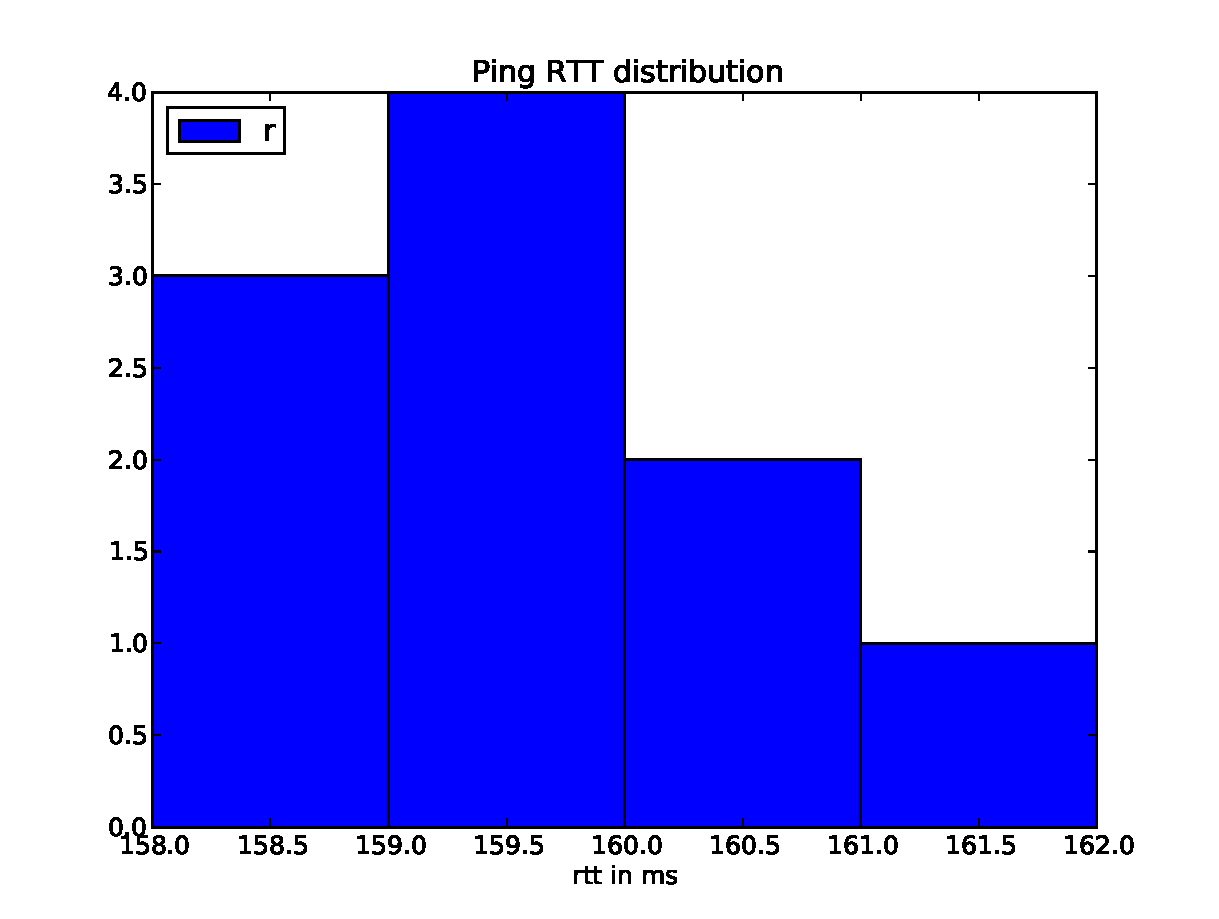
\includegraphics[height=6cm, width=7cm]{ping_distribution.pdf}  
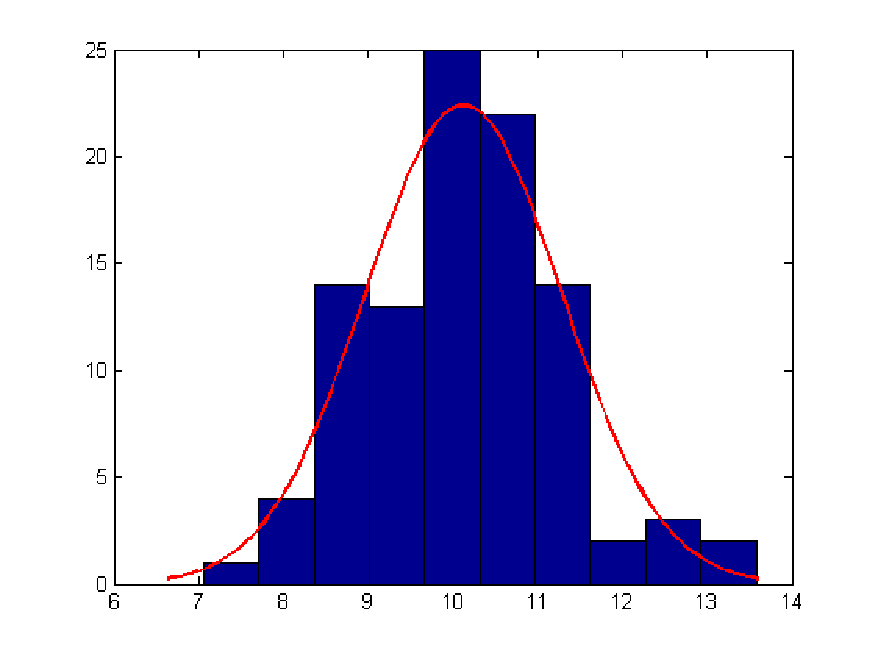
\includegraphics[height=5.5cm, width=7cm]{histo_gauss.pdf}
\end{columns}
\end{pyframe}

\subsection{Deviation}
\begin{pyframe}{Standard Deviation: scipy}
\begin{columns}
\column[t]{.4\textwidth}

\begin{itemize}
\item Standard deviation or $\sigma$ formula is {\large  $\sigma^{2}(X) := \frac{ \sum(x-\bar{x})^{2} }{n} $ }
\item $\sigma$ tells if $\delta$ is fair or not, and how much the mean ($\bar{x}$) is representative
\item \pymodule{matplotlib.mlab}.normpdf is a smooth function approximating the histogram
% Gauss function smoothly approximates the histogram {\Large 
%	$ \frac{n}{\sigma \sqrt{2\pi}}e^{-\frac{1}{2}  \big( \frac{x-\bar{x}} {\sigma} \big)^{2} } $ 
%} 
\end{itemize}

\column[t]{.6\textwidth}
\begin{pycode}
from scipy import std, mean
fair = [1, 1] # chickens
unfair = [0, 2] # chickens
assert mean(fair) == mean(unfair)

# Use standard deviation!
std(fair) # 0
std(unfair) # 1

\end{pycode}
\end{columns}
\end{pyframe}


\begin{pyframe}{Simple processing: scipy}
Check your computed values vs the $\sigma$ returned by ping 
(didn't you notice ping returned it?) 
\begin{pycode*}{escapeinside=||}
"""goal: remember to convert to numeric / float
   goal: use scipy
   goal: check stdev"""
from scipy import std, mean # max,min are builtin
rtt = ping_rtt()

print(max(rtt), min(rtt), mean(rtt), std(rtt))

\end{pycode*}
%fmt_s = 'stdev: {}, mean: {}, min: {}, max: {}'
%rtt_std, rtt_mean = |\pyver{std}|(rtt), |\emph{mean}|(ping_rtt)
%rtt_max, rtt_min = max(rtt), min(ping_rtt)
%print(fmt_s.format(rtt_std, rtt_mean, rtt_max, rtt_min))
\end{pyframe}

\begin{pyframe}{Time Distributions: Exercise}
\begin{itemize}
\item Parse the \href{https://github.com/ioggstream/python-course/blob/master/python-for-sysadmin/data/maillog}{provided maillog} in ipython using its ! magic and get an hourly email $\delta$
\item Expected output: 
\begin{pycode}
time_d = {  # mail delivered (removed) between
    0: xxx  #  00:00 - 00:59
    1: xxx  #  01:00 - 01:59
    ..
    }
\end{pycode}
\end{itemize}
\end{pyframe}
 
\iftrue
\begin{pyframe}{Time Distributions: Exercise Solution}
%def get_slot(ts):
%    n = int(ts[:2])
%    return n - (n%4)
\begin{pycode}
# deliveder emails are like the following 
#May 14 16:00:04 rpolli postfix/qmgr[122]: 4DC3DA: removed"
    
ret = !grep removed maillog # get the interesting lines

ts = ret.fields(2) # find the timestamp (3rd column)

hours = [ int(ts)  for x in ts ]
time_d = {x: count(x) for x in set(hours)}
\end{pycode}
\end{pyframe}

\fi 

\begin{pyframe}{Plotting distributions}
\begin{columns}
\column[t]{.6\textwidth}
\begin{pycode}
# To plot data..
from matplotlib import pyplot as plt
# and set the interactive mode
plt.ion()

# Plotting an histogram... 
frequency, bins, _ = hist(hours)

# .. returns a 
distribution = dict(zip(slots, 
    frequency))
\end{pycode}
\column[t]{.4\textwidth}
This server works mostly at night...
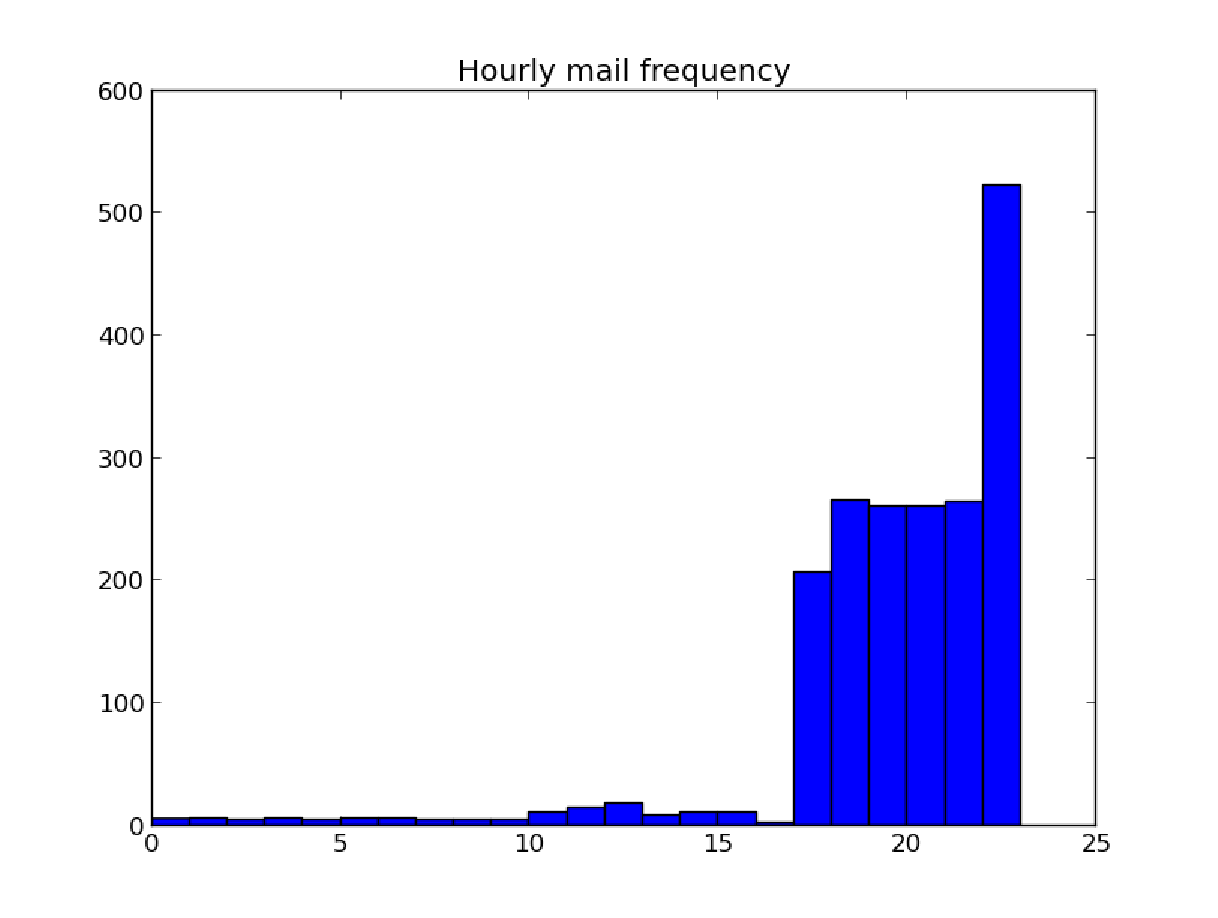
\includegraphics[width=6cm,height=5cm]{hourly_mail_d.pdf}
\end{columns}
\end{pyframe}

\begin{pyframe}{Size Distributions: Exercise}
\begin{itemize}
\item Create a size $\delta$ using \pyfunction{hist}(..., bins=...)
\item Hint: help(hist)
\begin{pycode}
size_d = {  # mail size between
    0: xxx  #  0 - 10k
    1: xxx  #  10k - 20k
    ..
    }
\end{pycode}
\item Homework: Use the size $\delta$ to find size\_mean and size\_sigma and compare with $\sigma$ and mean evaluated from the original data-series
\end{itemize}
\end{pyframe}



\begin{pyframe}{\pyoptional{Simulating data with $\sigma$ and $\bar{x}$}}
Mean and a stdev are useful starting point to simulate data using the gaussian distribution.
\begin{pycode*}{escapeinside=||}
# A mail load generator creating attachments of a given size...
from random import gauss
mail_size = gauss(mean, sigma_s) # a random number

# and use time_d to simulate the load during the day
from time import localtime
hour = localtime().tm_hour
mail_per_minute = time_d[hour] / |\pyver{60}| # minutes in hour
\end{pycode*}
\end{pyframe}



\subsection{Correlation}
\begin{pyframe}{Linear Correlation}
\begin{columns}
\column[t]{.6\textwidth}
\begin{pycode}
# Let's plot the following datasets
#  taken from a 4-hour distribution
mail_sent = [1, 5, 500, 250, 100, 7] 
kB_s = [70, 300, 29000, 12500, 450, 500]

# A scatter plot can suggest relations 
#  between data
plt.scatter(mail_sent, kB_s)





\end{pycode}
\column[t]{.4\textwidth}
\footnotesize
Correlating Mail and Thruput
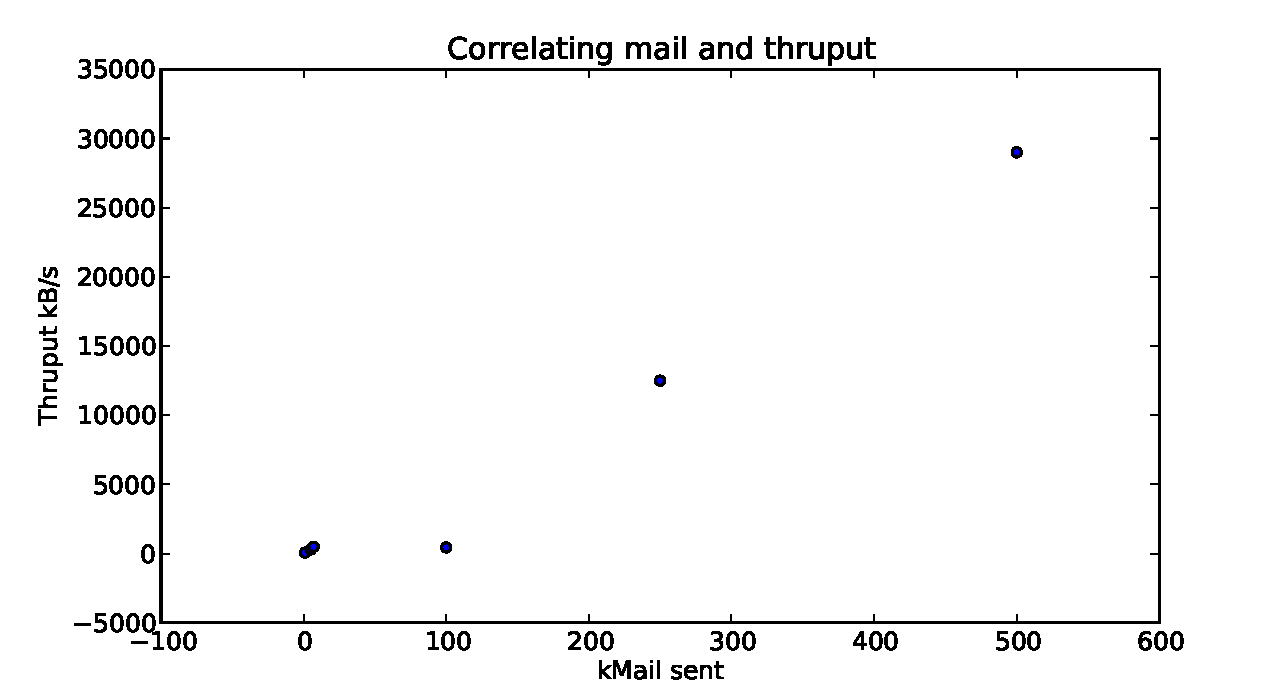
\includegraphics[height=5cm,width=6cm]{scatter_mail.pdf}
\end{columns}
\end{pyframe}


\begin{pyframe}{Linear Correlation}
The Pearson Coefficient $\rho$ is a relation indicator. 
\begin{description}
\item[0]  no relation
\item[1]  direct relation (both dataset increase together)
\item[-1]  inverse relation (one increase as the other decrease) 
\end{description}
\begin{equation}
\rho(X,Y) = \frac{
    \big(\sum (x-\bar{x})(y-\bar{y}) \big)
    }{
    \sqrt{\deltasumsq{x}}\sqrt{\deltasumsq{y}}
}
\end{equation}
\begin{pycode}
from scipy.stats.stats import pearsonr
ret = pearsonr(mail_sent, kB_s)
print(ret)
>(0.9823, 0.0004)
correlation, probability = ret
\end{pycode}
\end{pyframe}

\begin{pyframe}{You \emph{must (scatter) plot!}}
\LARGE
\begin{center}
$\rho$ does not detect non-linear correlation \\
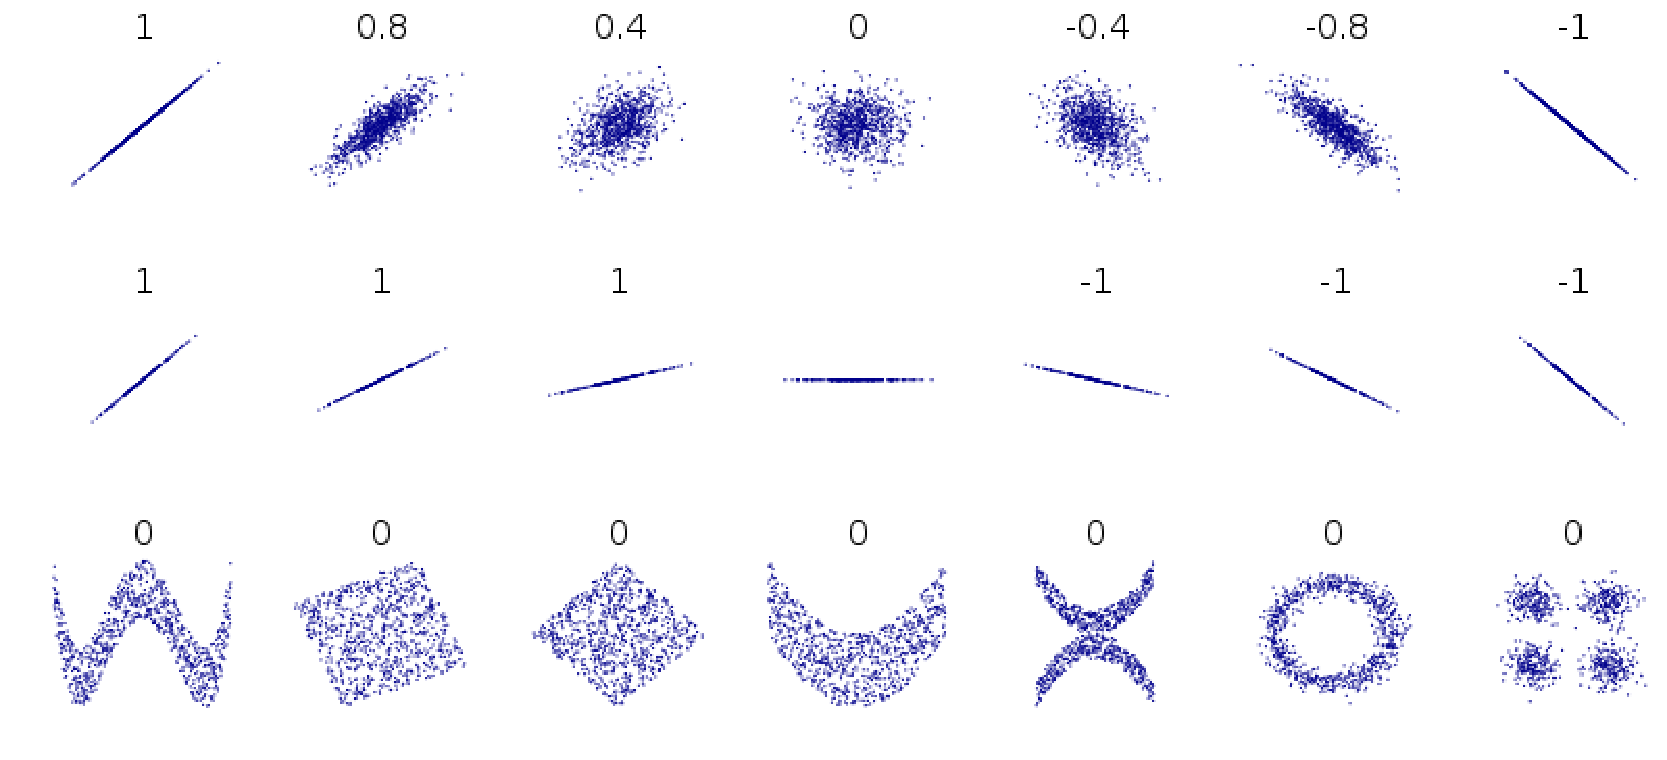
\includegraphics[width=.8\textwidth]{correlation.pdf} \\
\end{center}
\end{pyframe}


\begin{pyframe}{Combinations } % \dbinom{n}{k}}
\begin{columns}
\column[t]{.6\textwidth}
\begin{pycode}
# Given a table with many data series
from course import table
table = {...
  'cpu_usr': [10, 23, 55, ..],
  'byte_in': [2132, 3212, 3942, ..], }

# We can combine all their names with
from itertools import combinations
list(combinations(table,2))
>[('swap_in', 'cpu_sys'),
 ('swap_in', 'csw'),  ('cpu_sys', 'csw')... ]








\end{pycode}
\column[t]{.3\textwidth}
Combinating 4 suites, 2 at a time.\\
\begin{center}
\\
\hearts \spades \\
\hearts \clubs \\
\hearts \diamonds \\
\spades \clubs \\
\spades \diamonds \\
\clubs \diamonds \\
\end{center}
% complex image with 5-3-combination
%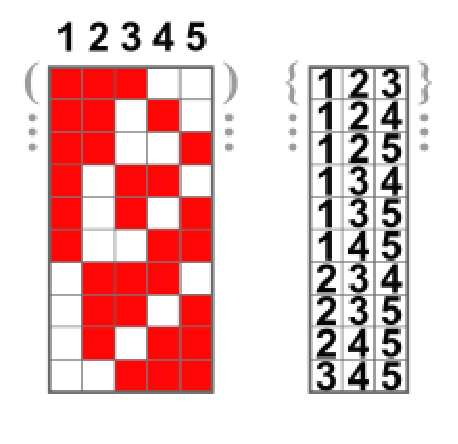
\includegraphics[width=4cm]{combinations_3.pdf}
\end{columns}
\end{pyframe}


\begin{pyframe}{Netfishing correlation}
We can try every combination between data series and check if there's some $\rho$.
\begin{pycode}
for k1, k2 in combinations(table, 2):
  corr, probability = pearsonr(table[k1], table[k2])
  if corr < 0.5:
    # I'm *still* not interested in data under this threshold
    continue
  print("linear correlation between {} and {} is {}".format(
    k1, k2, corr))

\end{pycode}
\end{pyframe}

\subsection{Plotting Time}
\begin{pyframe}{Correlating I/O and Context Switch}
{\footnotesize Now we'll generate some correlation plots from $table$ data, like this one.}
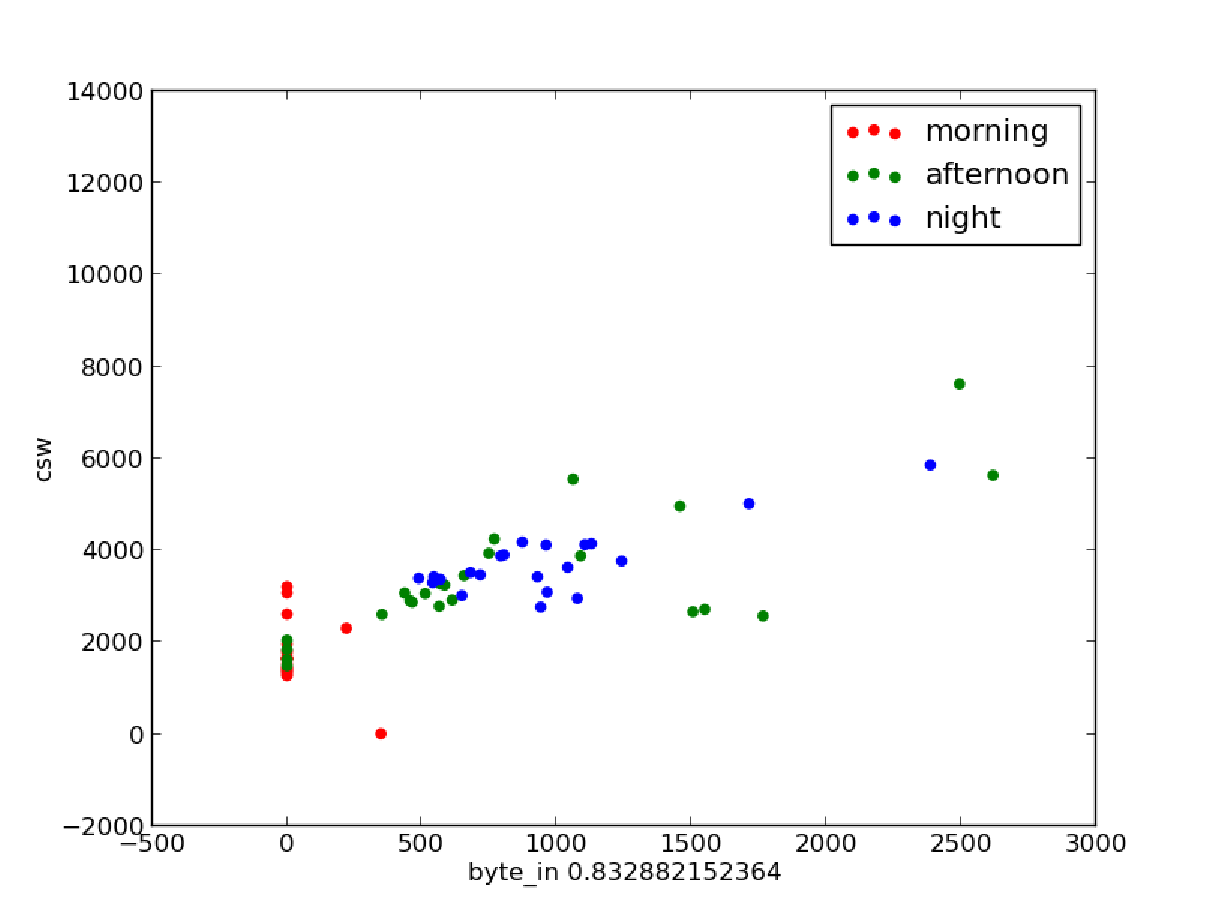
\includegraphics[height=6cm,width=14cm]{byte_in_csw.pdf}
\end{pyframe}


\begin{pyframe}{Netfishing correlation II}
\begin{pycode}
# create all combined plot
for k1, k2 in combinations(table, 2):
    corr, probability = pearsonr(table[k1], table[k2])
    plt.scatter(table[k1], table[k2])

    # 3 digit precision on title
    plt.title("R={:0.3f}".format(corr))
    plt.xlabel(k1); plt.ylabel(k2)

    # save and close the plot
    plt.savefig("{}_{}.png".format(k1, k2)); plt.close()
\end{pycode}
\end{pyframe}


\begin{pyframe}{Mark time with colors}
\begin{pycode*}{escapeinside=||}
# Use 3 colors to mark time-slots
from itertools import cycle
colors = cycle('rgb') # Red Green Blue
my_list = range(10)

# then import a function to chunk datasets
from course import in_chunks
in_chunks(my_list, size=4)) # returns a <generator object ...>
list(_) # ... which iterates to...
> [[0, 1, 2, 3], # Plotted in Red
   [4, 5, 6, 7], # ..Green
   [8, 9]]       # ..Blue 
\end{pycode*}
\end{pyframe}

\begin{pyframe}{Mark time with colors}
\begin{pycode*}{escapeinside=||}
# Get combined data directly via $\pyver{items}$
for (k1, v1), (k2, v2) in combinations(table.|\pyver{items}|(), 2):
    corr, probability = pearsonr(v1, v2)

    # Two nice generators
    time_chunked = zip(in_chunks(v1, size=8*3600),
                      in_chunks(v2, size=8*3600))
    [plt.scatter(t1, t2, color=|\pyver{next(colors)}|) # iterate colors!
        for t1, t2 in time_chunked]

    # save and close the plot
    plt.savefig("timed_{}_{}.png".format(k1, k2)); plt.close()
\end{pycode*}
\end{pyframe}





\section{End}
\begin{pyframe}{That's all folks!}
\begin{center}
Thank you for the attention! \\\\
\insertauthor
\end{center}
\end{pyframe}

\end{document}
